\chapter{Internship at Bosch}\label{ch:bosch}
\minitoc
This chapter is somewhat independent from the rest of this thesis and summarizes a voluntary internship I did at Bosch Hildesheim, Germany. However, many advancements of \acrshort{ml} algorithms are developed in the industry and gaining an insight into their development environment is of great benefit to academic research. At Bosch I was part of the corporate research department focusing on unsupervised pre-training for computer vision (\acrshort{cv}) algorithms. Specifically, I was tasked with developing and testing self-supervised learning algorithms for object detection. Due to the independence of this chapter from the others, I will give a brief introduction to deep learning object detection algorithms and self-supervised pre-training algorithms before describing my research at Bosch.

During my 4 month internship I managed to test a framework originally presented in \cite{Wei:2021aaa} on data used internally at Bosch. Additionally, I experimented with multiple new and original ideas targeted at improving the original framework for the application at Bosch. My time at Bosch resulted in a total of 4 invention reports, one of which will be discussed below. The others are either too far from the core topics of this thesis or are not published yet.

\section{Basics of Object Detection}
Traditionally, \acrshort{cv} challenges like the \acrshort{ilsvrc} have mainly focused on image classification. The task in image classification is to provide a single label to an image. The famous ImageNet dataset contains more than $21\,000$ classes and 14 million images \cite{Fei-Fei:2022aaa}. In object detection the task is to locate and annotate objects in an image. So rather than providing one global label to the entire image, the algorithm needs to specify one or multiple regions and apply a label to every one of them.

Once a good image classifier is available, getting an accurate object detector is in principal not too difficult. Theoretically, the classifier can be applied to each possible sub-region of the image to get a label. When the image classifier is setup such that it has a garbage class that is used for all images that do not contain any object, it would be able to detect and correctly annotate objects in an image. However, this direct approach is prohibitively computationally expensive, due to the factorial growth of sub-regions with the dimensions of the input image. To reduce that cost at the price of accuracy, one can instead use pre-determined regions in the image and classify those. An alternative is to use a fast algorithm to filter out the majority of uninteresting regions with low accuracy and only classify the remaining ones.

Before an overview of the evolution of deep learning object detection algorithms is given, a few core concepts have to be defined. First, the output of an object detector in the context discussed here is a rectangular bounding box of an object, whose sides are parallel to the edges of the image. Each bounding box has to be classified into one of $N+1$ categories, where $N$ is the number of object classes. The last class is the background class, that represents non-detections. To quantify how well a predicted bounding box aligns with a labeled box, a quantity known as the \emph{intersection over union} (\acrshort{iou}) is commonly used. It is defined as the area of the intersection of two rectangles divided by the area of their union. To quantify the performance of an object detection algorithm, the most common metric is the \emph{mean average precision} (\acrshort{map}). The \emph{precision} is the number of true positive detections divided by the number of total detections. It measures how likely a detection is to be a true positive and depends on the requirement for how well a bounding box has to be aligned with the ground truth to be considered a true positive, i.e. it depends on \acrshort{iou} requirements. The \acrshort{iou} also influences how likely a ground truth is to be recovered by the algorithm. This is measured by the \emph{recall}, which is the number of true positives divided by the number of ground truths. Since both the precision as well as the recall are a function of the \acrshort{iou}, they can be plotted against one another. The average precision, confusingly, is defined as the area under the precision-recall curve~\cite{Yohanandan:2020aaa}. The \acrshort{map} averages the average precision of all classes.

It is common to divide the architecture of an object detection \acrshort{nn} into two parts. Usually, a network pre-trained on image classification data is used to produce a feature map. This part of the object detection network is known as the \emph{backbone}. To adjust the output of the backbone to object detection and to produce the desired bounding boxes and classifications additional networks are attached to the backbone. These are known as \emph{heads} and often fine tuned on comparatively smaller amounts of object detection data sets.

The first major deep learning based object detection algorithm is known as R-CNN~\cite{Girshick:2013aaa} and selects regions of interest using the traditional algorithm ``selective search''~\cite{Uijlings:2013aaa}. Afterwards, it crops the proposed regions from the input image, projects them to a fixed size, and applies the then state-of-the-art AlexNet~\cite{krizhevsky:2012} to create fixed-size feature maps. In a third step, each feature map is evaluated by \acrshort{svm}s to find the class for the proposed region, where one class is a background class. The algorithm is trained, by first training the AlexNet on an image classification task. In a next step, the network is fine tuned on an object detection dataset. For this stage of training, the last layer of the AlexNet is replaced by a $N+1$ dimensional dense layer, where $N$ is the number of object classes and the additional output is used for background detections. For each image of the training set a selective search is used to propose regions of interest, which are then compared to the ground truth boxes. Proposed regions with an \acrshort{iou} $\geq 0.5$ with a ground truth box are defined as positive boxes and the rest are defined as negative boxes, i.e. background. From the proposed regions $32$ positive boxes and $96$ negative boxes are sampled, warped, and used as training data for fine tuning. In a final step, the last layer of the fine tuned network is discarded and one \acrshort{svm} is trained for each class. The resulting method outperformed previous existing methods by almost $20\%$ in \acrshort{map}~\cite{Girshick:2013aaa}.

The follow-up of R-CNN is Fast R-CNN~\cite{Girshick:2015aaa}. It still uses the selective search algorithm to generate region proposals. However, the network was upgraded to a VGG16 network~\cite{Simonyan:2014aaa} that was pre-trained on image classification data. Instead of applying it to different warped sub-regions of the image, the image is now processed only once as a whole. The proposed regions are then used to select parts of the resulting feature map, which are pooled to a fixed size using a process called RoIPooling. It also replaces the \acrshort{svm}s by a fully connected \acrshort{nn}, which has two outputs. One is the previous classification into $N+1$ classes. The other outputs 4 values, which are used to adjust the bounding box proposed by the selective search. Fine tuning is a lot easier than for R-CNN, as the entire network can be trained as a whole using standard deep learning optimizers. It improves over the original R-CNN by more than $15\%$ in \acrshort{map}~\cite{Girshick:2015aaa}.

The final version of R-CNN I want to briefly discuss here is Faster R-CNN~\cite{Ren:2015aaa}. It replaces the selective search region proposal algorithm by a \acrshort{nn}, thus making every part of the object detection pipeline a deep learning model. This \acrshort{nn} is called the region proposal network (\acrshort{rpn}) and introduces the concept of anchors. The \acrshort{rpn} processes its input to create a feature map, where each pixel is associated with a region in the input image. The size and shape of the region is the same for every pixel, but the location shifts such that the full image is covered. The regions are called \emph{anchors}. To have anchors of different sizes and aspect ratios, the output of the \acrshort{rpn} has multiple channels, where each can be associated with a different anchor size. The association is only learned and does not necessarily have to resemble the receptive fields of the pixels. For each anchor, two output values are produced; one is a binary classification into background/foreground, and the other are four values that adjust the location and size of the anchor. The remaining architecture is equivalent to that of Fast R-CNN~\cite{Girshick:2015aaa}. During inference, input images are processed by a \acrshort{cnn} that produces a feature map, which is then fed to the \acrshort{rpn}. All regions that are classified as foreground by the \acrshort{rpn} are cropped from the feature map of the initial \acrshort{cnn} using the RoIAlign layer from Fast R-CNN~\cite{Girshick:2015aaa} and fed to a classifier. Training is a more complicated five step process. First, the backbone is pre-trained on image classification data. Next, the \acrshort{rpn} is trained to find correct region proposals. For this \acrshort{iou} thresholds are chosen to select positive and negative anchor examples. The entire network, i.e. backbone and \acrshort{rpn}, is trained using a form of \acrshort{sgd}. The resulting \acrshort{rpn} is then used to generate region proposals to train a fresh Fast R-CNN, which uses the original pre-trained backbone weights. Once the Fast R-CNN is trained, the backbone is extracted, its weights are frozen, and a new \acrshort{rpn} is attached. This \acrshort{rpn} is trained again, where only the \acrshort{rpn} weights are optimized. Finally, the weights of the \acrshort{rpn} are also frozen, and the detection heads of the Fast R-CNN trained before are fine tuned using the new \acrshort{rpn} weights. It improves the \acrshort{map} over Fast R-CNN by about $2\%$ but more importantly increases evaluation speed. Where previous versions of R-CNN used multiple seconds to evaluate a single image, mainly limited by the selective search, Faster R-CNN allows the evaluation of $\approx 5$ images per second.

The different R-CNN variants are known as two stage detectors, as they propose regions of interest in a first step and classify each region in a second step. While this is a very accurate method, it is computationally expensive as each region of interest has to be processed on its own. To speed up object detection, single stage algorithms have been developed. Instead of only classifying regions of interest, they classify all of a set of pre-defined regions simultaneously.

One of the first major single stage object detectors that allowed to do object detection in real time and with accuracy comparable to Fast R-CNN was named You Only Look Once (\acrshort{yolo})~\cite{Redmon:2015aaa}. The network divides the input images into $S\times S$ cells. For each cell the network predicts $B$ bounding boxes and for all bounding boxes a confidence score is predicted. The confidence score gives an estimate of how likely it is that the box contains an object and how accurate the box is. Each cell is also associated with a probability score for all object classes, conditional on the predicted probability that the cell contains an object. The network architecture is also built up of a backbone with additional layers attached to handle object detection. The backbone is pre-trained on image classification data. To fine tune the architecture to object detection, ground truths are assigned to the grid cells which contain the center of the ground truth. The model can then be trained end-to-end, meaning that it is a single training loop. Since \acrshort{yolo} was introduced multiple improvements have been made and at the time of writing seven versions were released, of which only the first three are associated with the original authors~\cite{Redmon:2016aaa, Redmon:2018aaa, Bochkovskiy:2020aaa, Jocher:2022aaa, Li:2022aaa, Wang:2022aaa}.

Another single stage object detector, which many modern object detectors are based on, is the single shot multibox detector (\acrshort{ssd}) presented in \cite{Liu:2016aaa}. A variant of its architecture known as RetinaNet~\cite{Lin:2017aaa} was used in the experiments presented below. The core idea of \acrshort{ssd} is to adjust the architecture of the network to simultaneously process different object scales. The backbone of an object detector usually reduces the size of the feature map and increases the number of channels as the data passes through the network. The \acrshort{ssd} architecture attaches heads to intermediate layers of the backbone. The pixels from the output of the heads are then interpreted as belonging to anchor boxes in the original image in the same way Faster R-CNN did. The area covered by the anchor boxes is determined by the layer of the backbone at which the head was attached. Different channels in the output correspond to different aspect ratios of the anchor boxes. The training targets are created from the labeled data by \acrshort{iou} requirements of the ground truth boxes with the anchor boxes. Since the model is a one stage detector, it can be trained end-to-end. When it was released, it improved the \acrshort{map} over Faster R-CNN by almost $3\%$ while simultaneously being substantially faster to evaluate.

The \acrshort{ssd} architecture was improved over the years. The Retinanet~\cite{Lin:2017aaa} used a Resnet50~\cite{He:2015aaa} as backbone and attached a feature pyramid network (\acrshort{fpn})~\cite{Qiao:2021aaa}. The \acrshort{fpn} takes the different feature map scales used by \acrshort{ssd} and introduces additional connections that allow smaller scale features to be informed by larger scale features. For \acrshort{fpn}s a naming convention is used to specify how it is built. The different levels of the backbone from which features are extracted are called C1, C2, and so on. Once they have been processed by the \acrshort{fpn}, the outputs are called P1, P2, and so on, depending on which C-level they represent. Additionally, some \acrshort{fpn}s have a larger number of P-levels than C-levels. If that is the case, one can either build them on the output of the C-levels or the P-levels. See \autoref{fig:fpn} for a visualization. Another popular detector is called EfficientDet~\cite{Tan:2019aaa}, which uses an EfficientNet~\cite{Tan:2019aab} backbone and introduces a bi-directional \acrshort{fpn} allowing for information to flow from small scales to large scales.
\begin{figure}
	\centering
	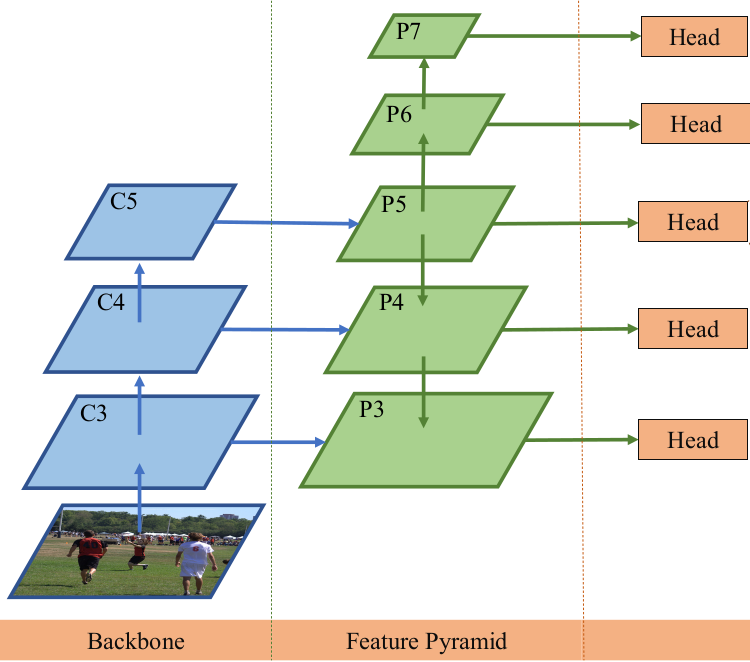
\includegraphics[width=0.6\textwidth]{chapters/internship/images/fpn.png}
	\caption[Feature pyramid network]{High-level overview of the structure of a \acrshort{fpn}. It shows a typical \acrshort{fpn} with levels P3 to P7, where P6 and P7 are built on top of P5. Arrows indicate connections, that can be of varying kind. Connections from P5 to P4 and P4 to P5 involve upsampling. This figure was taken from figure 2 in \cite{Tian:2019aaa}.}\label{fig:fpn}
\end{figure}


\section{Self-Supervised Pre-Training}\label{sec:ssl}
In this section I will introduce the concept of self-supervised learning (\acrshort{ssl}), focusing on a framework known as \emph{contrastive} learning. The goal of \acrshort{ssl} is to extract general information from raw data without labels. In the context of object detection, this data are images without any labeled objects. The hope is that the network will learn a general representation of images, which can then be fine tuned on comparatively few labeled training examples. This has the advantage of being computationally less expensive than full supervised learning, as plenty of raw data exists but labeling them is costly. Contrastive learning uses positive and negative pairs, where in the context of \acrshort{cv} positive pairs are usually different augmentations of the same image and negative pairs are augmentations of different images. The loss in this framework then encourages positive pairs to be similar and negative pairs to be dissimilar. Below I will give a brief overview of a few recent works in this field.

A framework known as SimCLR (simple framework for contrastive learnong of visual representations) was introduced in \cite{Chen:2020aab}. It consists of two networks $f$ and $g$ that operate on images $x$. The network $f$ is the core network that after fine tuning is supposed to be an image classifier, network $g$ translates the output of $f$ into a latent representation $z$. For each input two different augmentations $\tilde{x}$ and $\tilde{x}'$ are constructed and the latent representations $z$ and $z'$ are generated. For a batch of size $N$ we define $\hat{z}_{2i}=z_i$ and $\hat{z}_{2i+1}=z'$. The networks are then trained as one using the loss function
\begin{equation}
L=\frac{1}{2N}\sum_{k=1}^N\left[l\lr{2k, 2k+1} + l\lr{2k+1, 2k}\right]
\end{equation}
where,
\begin{equation}\label{eq:simclr_contrastive_loss}
l\lr{i, j}=-\log\left[ \frac{\exp\lr{s_{i,j}/\tau}}{\sum_{k=1}^{2N}\lr{1-\delta_{ki}}\exp\lr{s_{i,k}/\tau}}\right]
\end{equation}
and
\begin{equation}\label{eq:simclr_cosing_similarity}
s_{i, j} = \frac{\hat{z}_i\cdot\hat{z}_j}{\norm{z_i}\norm{z_j}}.
\end{equation}
The numerator in \eqref{eq:simclr_contrastive_loss} represents the positive pairs, whereas the denominator represents the negative pairs. The loss is minimized, when the cosine similarity \eqref{eq:simclr_cosing_similarity} for the positive pairs is minimized and for the negative pairs is maximized. The authors of \cite{Chen:2020aab} find that strong augmentations of the images improve their framework substantially and that large batch sizes ($\geq 256$) are useful. After fine tuning the network, they achieve performance almost equal to a full supervised training on ImageNet data. In a follow-up paper the authors improve on the results by utilizing very large networks~\cite{Chen:2020aac} and noticing that the larger the pre-trained model the less impactful the number of labeled images for fine tuning.

The authors of \cite{Grill:2020aaa} improve on the performance of SimCLR by introducing two branches of the same architecture. They call their approach Bootstrap Your Own Latent (BYOL) and its main advantage is that the loss does not contain any negative examples. This greatly reduces the computational cost during training, as fewer computations are required per batch sample. Instead of feeding two augmentations of the image to the same network, they introduce a second network, which is identical in architecture the first, to process the second augmentation. This setup can be understood as a teacher-student setup. Only the student is optimized directly through gradient descent, the teacher is updated by an exponential moving average of the student parameters. This procedure is also known as applying a stop-gradient to the teacher. Finally, a third network $\phi$ is introduced that is hypothesized to project the output of the student to the output of the teacher. The teacher and student produce two outputs $z$ and $z'$ for every input image and its different augmentations $x$ and $x'$, i.e. $z=g_\text{T}\lr{f_\text{T}\lr{x}}$, $z'=\phi_\text{S}\lr{g_\text{S}\lr{f_\text{S}\lr{x'}}}$, where the subscripts T and S refer to the teacher and student, respectively. The networks $f$ and $g$ serve the same roles as for SimCLR. The loss is given by a \acrshort{mse}
\begin{equation}
L=\norm{g_\text{T}\lr{f_\text{T}\lr{x}} - \phi_\text{S}\lr{g_\text{S}\lr{f_\text{S}\lr{x'}}}}^2 + \norm{g_\text{T}\lr{f_\text{T}\lr{x'}} - \phi_\text{S}\lr{g_\text{S}\lr{f_\text{S}\lr{x}}}}^2.
\end{equation}

In \cite{Chen:2020aaa} the authors present the SimSiam framework, which combines the advantages of SimCLR with those of BYOL. Their approach trains on positive pairs only and uses a stop gradient as BYOL, but does not require an exponential moving average for the teacher. They also remove the network $g$ from both approaches and are left with the network $f$ and the projector $\phi$. This greatly simplifies the overall setup for \acrshort{ssl} training and as a consequence greatly reduces the required batch sizes. While their final performance after fine tuning is weaker than that of BYOL, they manage to use less resources, which makes SimSiam viable even on modest hardware. As loss they use a negative cosine similarity.

The final \acrshort{ssl} framework I want to introduce is Selective object Contrastive learning (\acrshort{soco}) proposed in \cite{Wei:2021aaa}. Previous \acrshort{ssl} frameworks were used primarily for image classification tasks and only adapted to object detection by utilizing the pre-trained backbones. \acrshort{soco} is a \acrshort{ssl} framework specifically designed for object detection, allowing to pre-train the backbone and heads of a Mask-RCNN~\cite{He:2017aaa}. Mask-RCNN is a special Faster-RCNN that creates a pixel mask for different objects, instead of just generating bounding boxes. The proposed method is guided by the BYOL paper in the sense that it uses the three networks $f_\text{S}$, $g_\text{S}$, and $\phi_\text{S}$ for the student branch and the two networks $f_\text{T}$ and $g_\text{T}$ for the teacher, as well as using a stop gradient for the teacher and an exponential moving average to update the teacher parameters. What is called ``student'' here is named ``online network'' and what is called ``teacher'' is named ``target network'' in \cite{Wei:2021aaa}. The network $f$ is a Resnet50~\cite{He:2015aaa} with a \acrshort{fpn} attached. The \acrshort{fpn} is defined as in \cite{Lin:2017aaa} with levels P2 to P5. To adapt the BYOL framework to object detection, \acrshort{soco} produces regions of interest using the selective search algorithm~\cite{Uijlings:2013aaa}. Based on the size and location of the region proposal a corresponding area in one of the feature maps is selected and turned into a fixed size output by a layer named RoIAlign, which was introduced in \cite{He:2017aaa}. It is a special form of RoIPooling~\cite{Girshick:2015aaa} that interpolates its values to better align the input and the output. The output of the RoIAlign is then processed by the head, before being fed into the networks $g$ and $\phi$. To induce scale invariance of the object detector, the augmentation of one image is required to create a crop of the input image and resize it to the original size. Also, a third augmentation is processed, which is a downsized version of the augmented image that was cropped and resized. The loss is the sum of the cosine similarities of the output from the first augmentation with the cropped and resized augmentation and the first augmentation with the downsized version. See \autoref{fig:internship_soco} for a visualization of the framework.
\begin{figure}
	\centering
	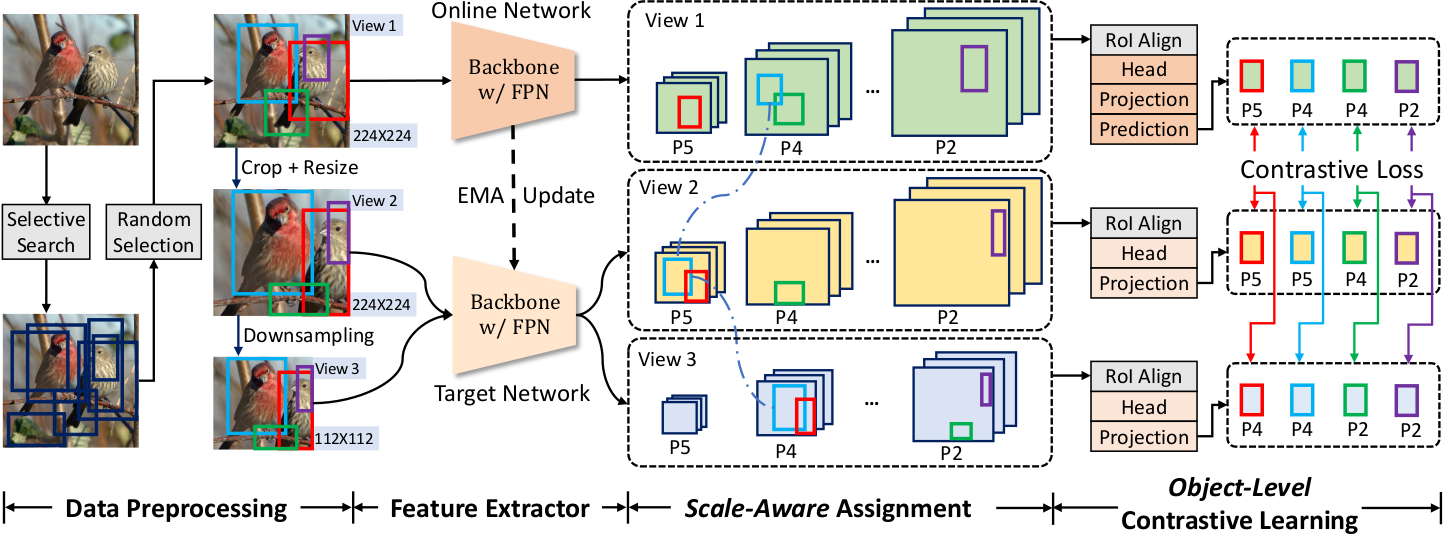
\includegraphics[width=0.98\textwidth]{chapters/internship/images/soco.png}
	\caption[Selective object Contrastive learning]{An overview of the \acrshort{soco} framework. What is called ``Online Network'' in the figure was described as student network in this chapter and what is called ``Target Network'' in the figure is the teacher network of this chapter. Different augmentations are used for view 1, 2, and 3. Different sized bounding boxes from the selective search are assigned different levels in the \acrshort{fpn}. This figure was taken from \cite{Wei:2021aaa} where it is figure 1.}\label{fig:internship_soco}
\end{figure}


\section{Research at Bosch}
At Bosch I was tasked with evaluating the usefulness of the approach called Selective object Contrastive learning (\acrshort{soco}) presented in \cite{Wei:2021aaa} to their existing object detection networks. The main challenges lay in two distinct points. First, the paper was mainly targeting two stage detectors, where the first stage samples possible regions of interest and the second stage classifies these regions. For the application that my work was targeting, anchor based single stage detectors are the prevalent approach, resulting in only portions of the architecture being able to be pre-trained using \cite{Wei:2021aaa}. Second, the code that was published~\cite{Wei:2022aaa} alongside the paper~\cite{Wei:2021aaa} needed to be validated and adapted for the networks, as well as the data used in the project.

Below I also present an adaption of the framework given in \cite{Wei:2021aaa} that I proposed to pre-train most of the single stage object detector architecture and eliminate the need to run a computationally expensive selective search \cite{Uijlings:2013aaa} before training. At the core it tries to encourage the network to create similar representations for two different augmentations of the same image. Only regions in the resulting feature maps that are present in both augmentations are compared. I evaluate the performance of a network pre-trained with this adaption, which I call \acrshort{ssdoco} (Single Shot Detector object Contrastive learning), against the same network pre-trained with the \acrshort{soco} framework.

\subsection{Introduction}
Training deep learning object detection algorithms is a difficult task. Creating classified bounding boxes as labels for the training data is far more time consuming, and therefore expensive, than creating labels that classify the entire image into a predetermined number of categories. For this reason, the interest in making un-labeled data usable for training purposes has picked up a lot of interest in the recent past~\cite{Chen:2020aab, Grill:2020aaa, Chen:2020aaa}. One of the most successful approaches so far has been a concept known as contrastive learning, which was introduced in \ref{sec:ssl}. Most of these algorithms focus on the task of image classification, where they have shown to improve performance even over full supervised training~\cite{Chen:2020aaa}. Although these algorithms are focused on image classification, they can still have a beneficial effect on object detection, as most object detection networks consist of a general backbone that aims to create a feature representation and an object detection specific part, like a feature pyramid network (\acrshort{fpn}), that tries to extract information at different scales. Afterward, classification and bounding box regression heads are attached to get the final output.

The backbone has traditionally been taken from state-of-the-art image classification algorithms~\cite{Chen:2020aab, Grill:2020aaa, Chen:2020aaa} and was always trained on image classification tasks. It is, therefore, reasonable to believe that \acrshort{ssl} pre-training algorithms devised for image classification may improve object detection algorithms, simply by improving the classification performance of the backbone.
On the other hand, object detection datasets are often different from image classification datasets. In image classification one commonly has images showing only a single object. For object detection training sets, these kinds of images are rare, and most images show multiple objects. Furthermore, additional parts of the object detection architecture, such as \acrshort{fpn}s or the detection heads, cannot be initialized from pure backbone pre-training and have to be trained from scratch on limited labeled data. To this end, it may be beneficial to develop pre-training algorithms that are tailored toward object detection, for instance by using contrastive loss functions that encourage similarity only in regions where the same objects are shown.

One of the first works presenting a \acrshort{ssl} framework that focuses on object detection is the \acrshort{soco} approach given in \cite{Wei:2021aaa}. Their goal was to pre-train the full architecture of a Mask-RCNN~\cite{He:2017aaa} that learned object level representations rather than global representations of the image. This means that rather than learning to produce similar feature maps of two different augmentations for the entire image, it focusses on producing similar representations only in regions where objects are likely to be present.

To select regions in which objects are likely to be present, \acrshort{soco} preprocesses the entire training set using a selective search \cite{Uijlings:2013aaa}, which is a generic algorithm that proposes regions of interest. This stage is computationally expensive but has to be executed only once per dataset. Whenever an image is used for training, a subset of the proposed regions is randomly selected.

In a next step, the two different augmentations of the input image are given to the two branches of their network. Both branches have the same architecture and mainly use a ResNet50 backbone~\cite{He:2015aaa} with a \acrshort{fpn}~\cite{Qiao:2021aaa}. For each selected and proposed region, the feature map that best matches the scale of the bounding box is selected and the part that corresponds to the feature map is cropped out. It is then passed to a RoIAlign layer which was introduced in\cite{He:2017aaa} to create a fixed size feature map. This can subsequently be processed by a detection head. The output of this detection head is further processed by additional layers aimed to project the output of the two branches into the same space. Finally, the output of one branch is processed by a final prediction module, that tries to translate the output of one branch to the output of the other branch. Afterward, the outputs of the two branches are compared by a cosine-similarity loss~\cite{Wei:2021aaa}.

The \acrshort{soco} framework allows to pre-train most of the Mask-RCNN architecture; backbone, \acrshort{fpn}, and classification heads. In fact, it can be easily adopted to pre-train most two stage detectors. However, adopting it to one stage detectors is not trivial. One stage detectors do a classification and bounding box regression for a fixed number of pre-determined locations in an image. Since all positions must be classified, selecting only a few of them for comparison has the potential to severely diminish the final performance.

To adapt the \acrshort{soco} framework to single stage detectors we propose \acrshort{ssdoco} (Single Shot Detector object Contrastive learning). Instead of comparing only select regions, \acrshort{ssdoco} compares compatible regions. One of the core principles of \acrshort{soco} is that one branch receives a cropped part of the original image as input to induce positional and scale invariance. \acrshort{ssdoco} uses the same concept but changes how the loss is constructed. It sums the cosine similarity loss of all compatible feature maps by cropping and interpolating the feature maps at different levels of the feature pyramid. This change allows us to effectively pre-train the entire single shot object detector, aside from the final layers.

\subsection{Methods}
We use a Retinanet~\cite{Lin:2017aaa} with a ResNet50~\cite{He:2015aaa} as backbone for our single stage object detector. The feature pyramid contains levels P3 to P7, where P6 is built from C5. For pre-training we use a single head consisting of 4 stacked convolutional layers with a kernel size of 3, 256 channels, and \acrshort{relu} activations. This architecture outputs 5 distinct feature maps of different scales. For fine-tuning both the classification head and the regression head are initialized with the weights from the single head during pre-training.

The \acrshort{ssdoco} framework follows the teacher-student model, where only the student is optimized directly using a gradient based optimizer and the teacher is updated through an exponential moving average of the student network parameters. Note that what we call the student is the ``online'' network in \cite{Wei:2021aaa} and what we call teacher is there known as the ``target'' network.

Both branches have multiple components. The student is composed of the model that should be trained, an alignment stage described below, a projector network, and a predictor network. The teacher is built the same way but does not contain a predictor network. Both the model as well as the projector of the teacher are updated by an exponential moving average of the student model and neither receive gradient updates. See \autoref{fig:internship_ssdoco} for a visualization of the framework.
\begin{figure}
	\centering
	\pgfdeclarelayer{bg}    % declare background layer
\pgfsetlayers{bg,main}  % set the order of the layers (main is the standard layer)
\begin{tikzpicture}[square/.style={regular polygon,regular polygon sides=4, draw, minimum width=2.4cm, fill=white}]
    \pgfmathsetmacro{\vsepa}{0.35}
    \node (img1) {Img 1};
    \node[below=2.4cm of img1] (img2) {Img 2};

    \node[square, right=.8cm of img1] (bbs) {BB};
    \node[square, right=.8cm of img2] (bbt) {BB};

    \node[square, right=\vsepa cm of bbs] (fpns) {\acrshort{fpn}};
    \node[square, right=\vsepa cm of bbt] (fpnt) {\acrshort{fpn}};

    \node[square, right=\vsepa cm of fpns] (as) {Align};

    \node[square, right=\vsepa cm of as] (projs) {Proj.};
    \draw (fpnt -| projs) node[square] (projt) {Proj.};

    \node[square, right=\vsepa cm of projs] (pred) {Pred.};

    \coordinate (h1) at ($(projs)!0.5!(projt)$);
    \node (contrast) at ($(h1 -| pred.east)+(.4, 0)$) {Contrast};

    \draw[->] (img1.south) -- (img2.north);
    \node[text width=2cm] at ($(img1.south)!0.5!(img2.north)+(1.2, 0)$) {Crop +\newline Resize};

    \draw[->] (bbs.south) -- (bbt.north);
    \node at ($(bbs.south)!0.5!(bbt.north)+(0.6, 0)$) {EMA};

    \draw[->] (fpns.south) -- (fpnt.north);
    \node at ($(fpns.south)!0.5!(fpnt.north)+(0.6, 0)$) {EMA};

    \draw[->] (projs.south) -- (projt.north);
    \node at ($(projs.south)!0.5!(projt.north)+(0.6, 0)$) {EMA};

    \draw[->] (img1.east) -- (bbs.west);
    \draw[->] (bbs.east) -- (fpns.west);
    \draw[->] (fpns.east) -- (as.west);
    \draw[->] (as.east) -- (projs.west);
    \draw[->] (projs.east) -- (pred.west);
    \draw[->] (pred.east) -| (contrast.north);

    \draw[->] (img2.east) -- (bbt.west);
    \draw[->] (bbt.east) -- (fpnt.west);
    \draw[->] (fpnt.east) -- (projt.west);
    \draw[->] (projt.east) -| (contrast.south);

    \node (augs) at ($(img1.east)!0.5!(bbs.west)+(-0.1, 0.3)$) {Aug};
    \node (augt) at ($(img2.east)!0.5!(bbt.west)+(-0.1, 0.3)$) {Aug};

    \draw[->] (augs.north) -- ++(0, 1) -| (as.north);

    \begin{pgfonlayer}{bg}    % select the background layer
        \draw[rounded corners, dashed, red, fill=red, fill opacity=.2] ($(bbs.north west)+(-.1, .1)$) rectangle ($(pred.south east)+(.1, -.1)$);

        \draw[rounded corners, dashed, blue, fill=blue, fill opacity=.2] ($(bbt.north west)+(-.1, .1)$) rectangle ($(projt.south east)+(.1, -.1)$);
    \end{pgfonlayer}

    \node[red] at ($(projs.north)+(.5, .5)$) {\textbf{Student}};
    \node[blue] at ($(projt.south)+(-1.9, .3)$) {\textbf{Teacher}};

    \node[minimum width=2.cm, right=\vsepa cm of projt] (sg) {
        \begin{tikzpicture}[anchor=0]
            \draw (-0.42, -.5) -- (.18, .5);
            \draw (-.18, -.5) -- (.42, .5);
        \end{tikzpicture}
    };
    \node at ($(sg.south)+(-.1, -.1)$) {stop-grad};
\end{tikzpicture}
	\caption[SSDoCo framework]{An overview of the \acrshort{ssdoco} framework. ``Img 1'' is an input image and ``Img 2'' is constructed from it by cropping and resizing to the original resolution. Each image subsequently gets its own augmentation ``Aug'', before being passed through the backbone ``BB'' and the \acrshort{fpn}. The ``Align'' step selects and interpolates the parts of the feature maps that are visible in ``Img 2''. The networks ``Proj.'' and ``Pred.'' are the projection and prediction networks. Finally, the contrastive loss is computed for both branches and the gradient is propagated back through the student. The parameters of the teacher are updated as an exponential moving average ``EMA'' of the student parameters.}\label{fig:internship_ssdoco}
\end{figure}

The two branches receive different augmentations of the same image. We follow \cite{Wei:2021aaa} for the choice of augmentations, but do not construct a “View 3”. The exact transformations are listed in \autoref{tab:transformations_ssdoco}. The teacher receives a random sub-view of the input to the student, the area of which is randomly selected between $50\%$ and $100\%$. The sub-view is subsequently resized to the original image size using bilinear interpolation. To enforce symmetry, we swap the inputs of the student and teacher after the forward pass and compute the loss as a sum of both results.
\begin{table}
\begin{tabularx}{\textwidth}{|p{0.02\textwidth}|X|p{0.276\textwidth}|X|p{0.06\textwidth}|X|p{0.06\textwidth}|}
\hline
\# & Name & Description & \multicolumn{2}{c|}{Student} & \multicolumn{2}{c|}{Teacher}\\
\cline{4-7}
& & & Params & Prob & Params & Prob \\
\hline
1 & Resize & Resize smaller side to 224 pixels & $-$ & $1$ & $-$ & $1$ \\
\hline
2 & Crop & Random crop to 224x224 pixels & $-$ & $1$ & $-$ & $1$ \\
\hline
3 & Random Crop + Resize & Random square crop and resize to 224x224 pixels & $-$ & $0$ & scale from $0.5$ to $1$ & $1$ \\
\hline
4 & Horizonal Flip & Flip image horizontally & $-$ & $0.5$ & $-$ & $0.5$ \\
\hline
5 & Color Jitter & Apply various color transformations & brightness $0.4$\newline contrast $0.4$\newline saturation $0.2$\newline hue $0.1$ & $0.8$ & brightness $0.4$\newline contrast $0.4$\newline saturation $0.2$\newline hue $0.1$ & $0.8$ \\
\hline
6 & Grayscale & Convert image to Grayscale & $-$ & $0.2$ & $-$ & $0.2$ \\
\hline
7 & Gaussian Blur & Blur the image & sigma from $0.1$ to $2$ kernel size $15\times 15$ & $1$ & sigma from $0.1$ to $2$ kernel size $15\times 15$ & $0.2$ \\
\hline
8 & Solarize & Solarize image & Threshold $128/255$ & $0.2$ & $-$ & $0$ \\
\hline
9 & Norm & Normalize the input data & Mean: $0.5$\newline Std: $0.225$ & $1$ & Mean: $0.5$\newline Std: $0.225$ & $1$ \\
\hline
\end{tabularx}
\caption[Transformations]{The image augmentations used for the \acrshort{ssdoco} training. The ``Prob'' columns give the probability of applying the given transformation.}\label{tab:transformations_ssdoco}
\end{table}

For the loss we use a variant of cosine similarity, which we shift and scale to return values between 0 and 2. The loss is given by
\begin{equation}
L\lr{y_1, y_2} = 2 + \frac{1}{n}\sum_{i=1}^n\text{L2}\lr{y_1^i, y_2^i},
\end{equation}
where $y_x$ is the output of model $x$, and $y_x^i$ is output $i$ of model $x$. The function L2 is given by
\begin{equation}
\text{L2}\lr{y_1, y_2} = -2\frac{y_1\cdot y_2}{\norm{y_1}\cdot\norm{y_2}}.
\end{equation}
However, naively comparing the five different feature maps would yield inconsistent results, as the input images are at different scales and show different regions of the same image. For this reason, we compare only those feature maps that are on similar scale and project the feature maps that were derived on the full image onto the sub-region given to the other branch of the Siamese network.

The feature pyramid in the network is built such that the scale of the features double at each level. We, therefore, enumerate the five output feature maps from smallest scale (i.e. largest feature map) to largest scale (i.e. smallest feature map). We then compare feature map $j+i$ of the unscaled image with feature map $j$ of the scaled image, where $i$ is given by
\begin{equation}
i=\lfloor\log_2\lr{s}\rfloor,
\end{equation}
with $1/s$ being the scale chosen in the Random Crop + Resize transformation. The index $j$ ranges from $0$ to $n-i$, where $n$ is the number of feature maps, i.e. 5. Our settings are chosen such that $1<s<2$ and, therefore, $i=0$. Consequently, we always compare the same levels of feature maps and only have to take care of the projection.

For the projection we interpret each pixel of the feature map as if it is associated to an anchor box in the input image. We then transform the anchor box-coordinates in the scaled branch to their (sub-pixel) position in the un-scaled image. This process takes re-scaling, cropping boundaries, and horizontal flips into account. We then interpolate the feature map of the un-scaled branch at those transformed coordinates, to obtain a comparable grid. We use bilinear interpolation. Afterward the feature maps are flattened, and the cosine similarity loss described above is applied.

\subsection{Experiments}
All pre-training uses a set of $1.6$ million diverse unlabeled images taken from Flickr~\cite{Flickr:2022aaa}. The data set was created internally to test the influence of large data sets which show widely differing scenes that are not specific to the final domain the network should operate on.

Once the pre-training is finished, all networks are fine tuned on the same set of labeled data. This set is also sampled from Flickr and contains $5\,500$ images. For each epoch, $5\,000$ batches are randomly sampled from the set and the network is trained for $40$ epochs with a batch size of $8$ or $80$ epochs with a batch size of $4$, depending on memory limitations of the hardware.

To compare the performance, we report the log average miss rate (\acrshort{lamr}) averaged over all six classes. We use the Caltech protocol given in \cite{Dollar:2012aaa} to determine true and false positives. The miss rate is averaged over five different false positive rates, where the false positive rate is given in terms of false positives per image. The miss rate is the number of false negatives divided by the number of ground truth boxes. Averaging over multiple false positive rates gives a more stable estimate of the detector performance. Lower values of the log average miss rate indicate better performance.

As baseline we fine tuned the network from random initialization. We found that the minimum \acrshort{lamr} after 40 epochs was $\approx 53\%$. To find any improvement, this baseline has to be beaten. Furthermore, we used ImageNet pre-trained weights as initialization for the backbone only. The \acrshort{fpn} and heads were initialized randomly. In this setup we found a minimal \acrshort{lamr} of $\approx 33\%$.

\subsubsection{SoCo}
We adjusted the code published alongside the \acrshort{soco} paper~\cite{Wei:2022aaa} to use the Retinanet discussed above. However, we removed the heads from the Retinanet and only replaced the backbone and \acrshort{fpn}, as both components differ to the original implementation only in minor details. The greatest difference is the inclusion of the levels P6 and P7, which were dropped from the original work due to the size of the resulting feature maps. Our network uses the outputs $\left\{\text{P3}, \text{P4}, \text{P5}, \text{P6}, \text{P7}\right\}$. Consequently, we also had to adjust the awareness scales. We define object proposals of area within the range of $\left\{0-48^2,49^2-96^2,97^2-192^2,193^2-208^2,209^2-224^2\right\}$ pixels to $\left\{\text{P3}, \text{P4}, \text{P5}, \text{P6}, \text{P7}\right\}$, respectively. Due to hardware limitations we also had to lower the batch size to $64$ samples.

Before training, we applied the selective search to the entire training set. To reduce runtime, we resized all images such that the smaller side has a size of $224$ pixels, before applying selective search. Afterward, the boxes were scaled to match the original image size.

We pre-trained the architecture for $10$ epochs with a warmup of $1$ epoch using the same LARS optimizer~\cite{You:2017aaa} and settings as given in the \acrshort{soco} repository~\cite{Wei:2022aaa}. We found that the outputs of the network grow during pre-training. This forced us to not use mixed precision training during fine tuning and, therefore, reduce the batch size to $4$. This fine tuning seemed to be unstable and only converging occasionally. When the fine tuning converged, performance was on the order of a randomly initialized network.

To make sure that the architecture was not a problem, we changed the backbone and \acrshort{fpn} to match those cited in the paper~\cite{Wei:2021aaa}. We also changed the association of the area of proposals with \acrshort{fpn} levels back to the original implementation. However, pre-training and fine tuning showed the same problem as before, with the network converging only sometimes. Converged networks could not beat a random initialization during fine tuning.

When we fine tune the network, we only initialize those parts of the network that have had pre-training. The remaining weights and biases are initialized randomly. This means that the P6 and P7 levels are initialized randomly in our second experiment during fine tuning. In both cases, we tested initializing both the backbone and the \acrshort{fpn} as well as only the backbone. Neither option yielded any improvements over the other.

\subsubsection{SSDoCo}
To evaluate the SSDoCo approach, we tested multiple different ideas aimed at improving performance. All tests use the same backbone and \acrshort{fpn} of the Retinanet, but the projector and predictor were varied. We also experimented with different optimizers and regularization techniques.

Initially, following the architecture of SimSiam~\cite{Chen:2020aaa}, the projectors were removed and the predictors for the different feature maps were $1\times 1$ convolutions that only altered the channel dimension. We trained the network with the Adam~\cite{Kingma:2014aaa} optimizer. The transformation aligning the outputs was placed after the output of the predictor. These experiments showed that the output was continually growing, the longer we trained. This caused fine tuning to be unstable and diverge. Consequently, we introduced L2 regularization~\cite{Ng:2004aaa}, to reduce the numerical values of the weights and, thereby, the output. We also switched to the LARS~\cite{You:2017aaa} optimizer, following the recommendations of the \acrshort{soco} paper.

After these alterations, the network output stayed on average below 1. However, the loss quickly fell during the first few batches and continued to grow afterward. This problem was rectified by lowering the initial learning rate by an order of magnitude. The resulting algorithm trained smoothly but checking the outputs for different inputs revealed that the output was constant for different inputs.

We initially tried to force the network to avoid collapsing to constant outputs by introducing a new regularization term to the loss. This term penalizes low weight variance and is given by
\begin{equation}
L\lr{\theta}=\frac{1}{N}\sum_{i=1}^N\lr{s\text{Var}\left[\theta_i\right]+\epsilon}^{-1},
\end{equation}
where $s$ is a scale factor, $\epsilon$ is a small constant, and $\theta_i$ are the parameters of layer $i$. The function Var calculates the variance of the parameters. After some experiments we found that this regularization seems to solve the problem. However, fine tuning resulted in a network that is on par with a randomly initialized network.

To align the \acrshort{ssdoco} training more strongly with both the \acrshort{soco} training and previous \acrshort{ssl} pre-training experience, we introduced a projector using global average pooling, followed by two dense layers. The predictor was altered to consist of two dense layers, where the first is a bottleneck, i.e. having fewer neurons than its input and the subsequent output. We also moved the transformation aligning the outputs of the teacher and the student to take place between the Retinanet and the projector. So, the student is composed of a Retinanet, followed by the output alignment, the projector, and finally the predictor. The teacher network has the same structure but drops the predictor. Both the Retinanet and the projector of the teacher are updated through an exponential moving average of the student.

Aligning the setup with previous experience, the output dropped to expected small scales. However, fine tuning still did not produce a network that could beat a random initialization.

We also tried fine tuning all architectures by initializing only the backbone and \acrshort{fpn} of the network with the pre-trained weights. This had proven helpful in other scenarios. However, this could not improve fine tuning results either.

We had planned to test the influence of the batch size, the size of the bottleneck layer, and the influence of different data set sizes on the final performance of the algorithm. Due to a missing baseline, we could not perform these experiments.

Pre-training was carried out on four NVIDIA A6000 GPUs for a total batch size of $128$. Training for $10$ epochs on $1.6$ million images required about 4 days. We used a learning rate of $0.1$ and a momentum of $0.9$ in the LARS optimizer. We used the same weight decay implementation and settings as given in \cite{Wei:2022aaa}.

\subsection{Conclusions}
We have tested the \acrshort{soco} framework presented in \cite{Wei:2021aaa} and a custom extension of it – named \acrshort{ssdoco} – on a diverse dataset. Our goal was to pre-train a Retinanet for complex object detection tasks on a large unlabeled dataset and fine tune it on application specific data. The frameworks allowed to pre-train both the backbone as well as the \acrshort{fpn}, while the \acrshort{ssdoco} approach was envisioned to also allow pre-training of the detection- and classification-heads.

We found that neither of the two contrastive pre-training methods managed to produce network parameters that could beat a random initialization during a fixed fine tuning. Especially, the findings of \acrshort{soco} could not be reproduced on our data. We hypothesize that this could be due to two reasons. First, our datasets contain many objects, compared to MS Coco~\cite{Lin:2014aaa}, which was used in \acrshort{soco}. This could be challenging for a framework that tries to align object views. Second, limited hardware resources restricted the batch size we could use during pre-training to $64$ samples. The lowest batch size results are reported on in \cite{Wei:2021aaa} is $512$; a $8$ times increase over our setup.

The \acrshort{ssdoco} setup allowed us to train with a batch size of $128$. The training produced much more stable results, that managed to converge every time during fine tuning. However, the performance after fine tuning could not outperform random initialization. Given that the \acrshort{soco} framework, which the \acrshort{ssdoco} approach is loosely based on, did not produce positive results on our datasets, we believe it to be unlikely that \acrshort{ssdoco} will yield tangible performance benefits. However, other \acrshort{ssl} methods have already proven to be successful, which justifies further research in this area.
